% Compact chapter-local teaching panels; global theme is unchanged.
\newcommand{\VoltageIdea}[2]{\par\smallskip\begin{beamercolorbox}[sep=.8mm,wd=\linewidth]{block body}{\color{teal}\bfseries #1\par}#2\end{beamercolorbox}\par}

\begin{frame}[t]{The operator's question: how much PV can this feeder accept?}
\label{f:V01}
\small

\begin{columns}[T]
\column{.47\textwidth}
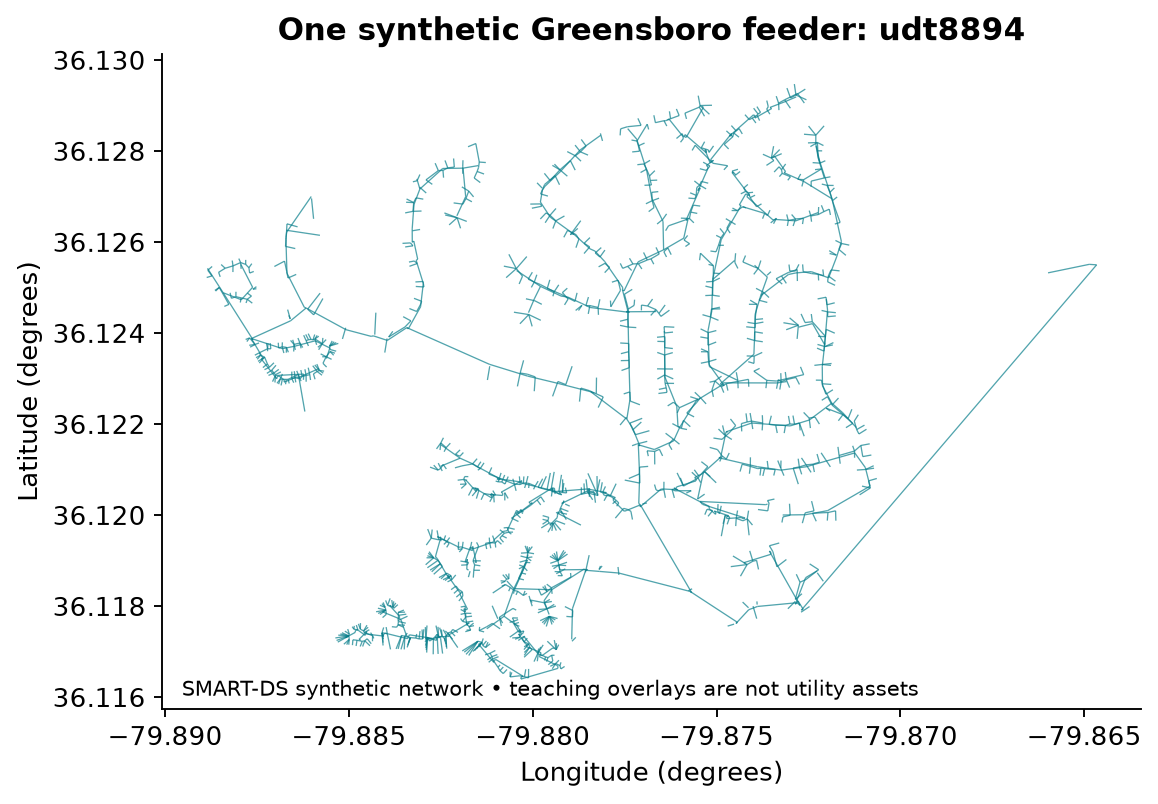
\includegraphics[width=\linewidth,height=3.75cm,keepaspectratio]{figures/feeder.png}
{\scriptsize One SMART-DS synthetic Greensboro feeder:\\ \texttt{uhs20\_1247--udt8894}.}
\column{.50\textwidth}
\VoltageIdea{An operating request}{Use available PV while keeping modeled voltages and currents within their limits.}
\medskip
\par\begin{tikzpicture}[x=1cm,y=1cm]
\node[draw=navy,thick,minimum width=1.1cm,minimum height=.8cm] (op) at (0,0) {\small Operator};
\node[box,text width=2.6cm] (rec) at (3.3,0) {Proposed inverter\\command + evidence};
\draw[arrow] (op)--node[above,font=\scriptsize]{request}(rec);
\node[font=\small,text=slate,align=center] at (1.7,-1) {A good answer explains\\what was checked and what was omitted.};
\end{tikzpicture}\par
\uncover<2->{\Question{Which could limit additional PV: voltage, current, or inverter capability?}
\Answer{Any of the three. We must inspect their margins together.}}
\end{columns}

\Source{\href{https://data.openei.org/submissions/2981}{SMART-DS synthetic distribution models}; Executed \texttt{Classroom\_Labs.ipynb}; \texttt{src/classroom\_labs.py}}
\Bridge{What physical path connects the PV inverter to the source?}
\note{The voltage chapter uses one SMART-DS synthetic Greensboro feeder, identified as uhs20\_1247--udt8894. It is not a model of the whole city or a live utility. Ask learners which information they still need before advising an operator: device availability, thermal ratings, voltage bounds, model coverage and permitted actions. The map establishes geographic context; it does not establish operational validity. Our numerical experiment uses a fleet command with two continuous variables. All recommendations remain advisory simulation outputs. This chapter moves from a familiar control problem to the reason for explicit agent handoffs: a recommendation should carry the evidence and assumptions that justify it.}
\end{frame}

\begin{frame}[t]{See the electrical path before choosing an algorithm}
\label{f:V02}
\small

\begin{center}
\par\begin{tikzpicture}[x=1cm,y=1cm]
\node[draw=navy,thick,minimum width=1.4cm,minimum height=.9cm,align=center] (src) at (0,0) {Source\\$V_s$};
\coordinate (b) at (6.8,0);
\draw[very thick,navy] (src.east)--(2.1,0);
\draw[thick,teal,fill=pale] (2.1,-.23) rectangle (4.6,.23);
\node[font=\small] at (3.35,.65) {Feeder impedance $r+jx$};
\draw[very thick,navy] (4.6,0)--(8.8,0);
\fill[navy] (b) circle (2pt);
\node[above,font=\small] at (b) {Bus voltage $V$};
\draw[very thick,navy] (8.8,0)--(8.8,-1.4);
\node[box] at (8.8,-1.8) {Local load};
\draw[very thick,navy] (b)--(6.8,-1.4);
\node[draw=teal,thick,fill=pale,minimum width=1.8cm,minimum height=.75cm] (inv) at (6.8,-1.8) {Inverter};
\node[draw=navy,fill=pale,minimum width=1.5cm,minimum height=.65cm] (pv) at (3.7,-1.8) {PV array};
\draw[arrow] (pv)--node[above,font=\scriptsize]{DC power}(inv);
\uncover<2->{\draw[arrow,draw=amber] (6.3,-1.25)--(6.3,-.15);
\node[font=\small,align=left,text=navy] at (4.9,-.75) {$p_{\rm PV}$\\$q_{\rm inv}$};}
\uncover<3->{\draw[arrow,draw=red] (4.5,.95)--(2.3,.95);
\node[above,font=\small,text=red] at (3.4,.95) {High PV can reverse power flow};}
\end{tikzpicture}\par
\end{center}
{\small $r$: resistance; $x$: reactance; $\mathrm{j}^2=-1$. $p_{\rm PV},q_{\rm inv}$: active/reactive inverter injection.}
\begin{columns}[T]
\column{.32\textwidth}\VoltageIdea{Voltage}{The line impedance turns power flow into a voltage change.}
\column{.32\textwidth}\VoltageIdea{Current}{Both active and reactive flow use current capacity.}
\column{.32\textwidth}\VoltageIdea{Inverter}{Active and reactive commands share one kVA rating.}
\end{columns}

\Source{\href{https://arxiv.org/abs/1406.3054}{Gan \& Low: three-phase distribution optimization (2014)}}
\Bridge{Why can absorbing reactive power reduce a high feeder voltage?}
\note{Begin at the source and follow the physical conductor to the load and inverter. The PV array supplies DC power; its inverter provides a controlled AC interface. The feeder impedance makes local voltage depend on both active and reactive flow. Under sufficiently high PV production, net active power can flow toward the source, which can raise downstream voltage. Reactive support is not free: it also changes current and consumes inverter capability. The picture is an explanatory single-branch abstraction, not the topology used by the full numerical model. Ask learners to point to the location of each measured quantity. This establishes a physical reference for the next sign-convention and arithmetic examples.}
\end{frame}

\begin{frame}[t]{Keep net demand and inverter injection signs distinct}
\label{f:V03}
\small

\begin{columns}[T]
\column{.48\textwidth}
\VoltageIdea{The feeder sees net demand}{Positive $P,Q$ mean net consumption downstream.}
\[
P=P_{\rm load}-p_{\rm PV},\qquad
Q=Q_{\rm load}-q_{\rm inv}.
\]
\par\begin{tikzpicture}
\node[box] (s) {Source};\node[box,right=2.0cm of s] (b) {Bus};
\draw[arrow] (s)--node[above,font=\scriptsize]{$P,Q>0$}(b);
\end{tikzpicture}\par
\medskip
{\small $P,Q$: net active/reactive power; $P_{\rm load},Q_{\rm load}$: demand; $p_{\rm PV},q_{\rm inv}$: inverter injections. Use one consistent power base.}
\column{.48\textwidth}
\uncover<2->{\VoltageIdea{The inverter absorbs reactive power}{$q_{\rm inv}<0$ increases net $Q$.}
\[
\Delta V\approx rP+xQ,\qquad V\approx V_s-\Delta V.
\]
\par\begin{tikzpicture}[x=1cm,y=1cm]
\node[box] (v) at (0,0) {High $V$};
\node[box] (q) at (2.5,0) {Absorb $Q$};
\node[box] (w) at (5,0) {Lower $V$};
\draw[arrow] (v)--(q);\draw[arrow] (q)--(w);
\end{tikzpicture}\par
\medskip
{\small For positive line reactance $x$, more net reactive consumption increases the approximate drop.}}
\end{columns}
\uncover<3->{\VoltageIdea{Physical tradeoff}{Lower voltage can require more current. We must check both.}}

\Source{\href{https://arxiv.org/abs/1406.3054}{Gan \& Low: three-phase distribution optimization (2014)}; illustrative single-branch linearization, not a feeder measurement}
\Bridge{Can we calculate that voltage change with three numbers?}
\note{State both sign conventions explicitly. The distribution line sees net demand: positive P and Q mean consumption downstream. The inverter uses an injection convention, so positive reactive injection reduces net reactive demand, while absorption means a negative inverter reactive command and increases net Q. For a conventional line with positive resistance and reactance, increasing net reactive demand increases the approximate voltage drop. The voltage expression is a small-drop per-unit teaching approximation around nominal voltage, not the full three-phase model. Use the arrows to distinguish these quantities before introducing the actual fleet parameter b. The physical tradeoff is that reactive absorption may reduce high voltage while increasing the magnitude of current.}
\end{frame}

\begin{frame}[t]{A small calculation: reactive absorption lowers high voltage}
\label{f:V04}
\small

\begin{columns}[T]
\column{.40\textwidth}
\VoltageIdea{Illustrative single branch}{All quantities are per unit on consistent bases.}
\[
V_s=1.04,\quad r=0.02,\quad x=0.04,
\]
\[
P=-0.60.
\]
{\small Negative $P$ means net PV export. $Q$ is net reactive consumption. This is arithmetic for intuition, not output from the Greensboro model.}
\medskip
\par\begin{tikzpicture}
\node[box] (s) {$V_s=1.04$};\node[box,right=1.2cm of s] (b) {$V=?$};
\draw[arrow] (s)--node[above,font=\scriptsize]{$r+jx$}(b);
\end{tikzpicture}\par
\column{.57\textwidth}
\[
V\approx V_s-rP-xQ.
\]
\uncover<2->{\VoltageIdea{No reactive absorption: $Q=0$}{
$V\approx1.04-0.02(-0.60)=1.052$ p.u.\\
\textcolor{red}{Above the illustrative 1.05 p.u. upper bound.}}}
\medskip
\uncover<3->{\VoltageIdea{Absorb reactive power: $Q=0.20$}{
$V\approx1.04+0.012-0.008=1.044$ p.u.\\
\textcolor{teal}{The voltage now passes that bound.}}}
\end{columns}

\Source{Illustrative arithmetic using a linear voltage-drop approximation; \href{https://arxiv.org/abs/1406.3054}{Gan \& Low: three-phase distribution optimization (2014)}}
\Bridge{Does passing the voltage bound mean the action is acceptable?}
\note{Give the audience time to compute the first voltage before revealing it. The source voltage is 1.04 per unit, the line resistance and reactance are 0.02 and 0.04 per unit, and net active export is 0.60 per unit. With zero net reactive demand, the linear approximation predicts a voltage rise to 1.052. Adding 0.20 per unit of reactive absorption creates a drop that reduces the estimate to 1.044. The example intentionally uses round numbers and a single branch, so it is neither a calibrated feeder result nor a validation of the three-phase adapter. Ask which sign in the equation explains the change. The next slide checks the current consequence of the same action.}
\end{frame}

\begin{frame}[t]{Voltage passes, but current can still fail}
\label{f:V05}
\small

\[
I\approx\frac{\sqrt{P^2+Q^2}}{V_s},\qquad
V_{\max}=1.05,\quad I_{\max}=0.60\ {\rm p.u.}
\]
{\small $I$: approximate current magnitude; $P,Q$: net power; $V_s=1.04$ p.u. fixed reference. The limits are illustrative.}
\medskip
\begin{center}
\begin{tabular}{lrrrrl}
\hline
Action & $P$ & $Q$ & $V$ & $I$ & Checks\\\hline
PV export only & $-0.60$ & $0$ & $1.052$ & $0.577$ & \textcolor{red}{Voltage fails}\\
\uncover<2->{Add absorption} & \uncover<2->{$-0.60$} & \uncover<2->{$0.20$} & \uncover<2->{$1.044$} & \uncover<2->{$0.608$} & \uncover<2->{\textcolor{red}{Current fails}}\\
\uncover<3->{Also reduce export} & \uncover<3->{$-0.55$} & \uncover<3->{$0.20$} & \uncover<3->{$1.043$} & \uncover<3->{$0.563$} & \uncover<3->{\textcolor{teal}{Both pass}}\\\hline
\end{tabular}
\end{center}
\medskip
\Question{Which action would a voltage-only checker mistakenly accept?}
\uncover<3->{\VoltageIdea{Why we need optimization and verification}{Balance active power, reactive effort and every declared limit. A single improved metric is insufficient.}}

\Source{Explicitly illustrative per-unit arithmetic; no measured or simulated feeder result}
\Bridge{How can a planner coordinate these tradeoffs across several forecast steps?}
\note{Carry the previous voltage example forward without changing its assumptions. The approximate current uses apparent-power magnitude divided by the fixed source-voltage reference. PV export alone gives acceptable current but excessive voltage. Reactive absorption fixes the voltage while increasing current slightly beyond the illustrative limit. Reducing the magnitude of active export then makes both checks pass in this approximation. The three rows isolate the tradeoff and explain why a good voltage result is not enough. All values are rounded and belong only to this single-branch arithmetic example. They are not the tutorial's actual MPC or SAC commands. Ask participants to name any additional checks still missing, including inverter capability and the validity of the model itself.}
\end{frame}

\begin{frame}[t]{The five stages turn an action into reviewable evidence}
\label{f:V06}
\small

\begin{center}
\par\begin{tikzpicture}[x=1cm,y=1cm]
\node[box,text width=2.05cm,minimum height=1.1cm] (a) at (0,0) {\textbf{Awareness}\\What is the case?};
\node[box,text width=2.05cm,minimum height=1.1cm] (p) at (2.7,0) {\textbf{Planning}\\What should we try?};
\node[box,text width=2.05cm,minimum height=1.1cm] (s) at (5.4,0) {\textbf{Simulation}\\What happens?};
\node[box,text width=2.05cm,minimum height=1.1cm] (v) at (8.1,0) {\textbf{Verification}\\Does it pass?};
\node[box,text width=2.05cm,minimum height=1.1cm] (o) at (10.8,0) {\textbf{LLM\\optimizer}\\What next?};
\draw[arrow] (a)--(p);\draw[arrow] (p)--(s);\draw[arrow] (s)--(v);\draw[arrow] (v)--(o);
\uncover<2->{\node[below=5mm of a,text width=2.2cm,align=center,font=\small] {Load, ratings,\\model scope};
\node[below=5mm of p,text width=2.2cm,align=center,font=\small] {MPC / SAC\\candidate $(a,b)$};
\node[below=5mm of s,text width=2.2cm,align=center,font=\small] {Voltages and\\branch currents};
\node[below=5mm of v,text width=2.2cm,align=center,font=\small] {PASS or reasons\\to reject};
\node[below=5mm of o,text width=2.2cm,align=center,font=\small] {One permitted\\refinement};}
\uncover<3->{\draw[arrow,draw=amber] (o.south) -- ++(0,-2.0) -| node[pos=.25,below,font=\small]{changed action: simulate and verify again} (s.south);}
\end{tikzpicture}\par
\end{center}
\VoltageIdea{The lesson from the arithmetic}{The optimizer may suggest reducing export. The numerical checker must establish whether that new command meets the declared limits.}

\Source{Executed \texttt{Classroom\_Labs.ipynb}; \texttt{src/classroom\_labs.py}; five-stage proposal architecture}
\Bridge{What does the model-based planner calculate?}
\note{Connect each stage to the physical tradeoff just calculated. Awareness establishes the source conditions, ratings, model scope and permitted actions. Planning proposes a command, using the appropriate numerical method. Simulation computes its consequences, while verification decides whether those consequences satisfy the contract. The language optimizer can select a permitted next trial, but the modified command has to return to the numerical stages. The actual tutorial uses MPC and SAC as candidate generators and model-specific power-flow adapters for checking. It does not require an LLM call in every stage. Deterministic computation remains essential. Ask learners to identify which stages repeat after changing only reactive absorption, and which evidence must be replaced.}
\end{frame}

\begin{frame}[t]{MPC uses a forecast, then commits only the first move}
\label{f:V07}
\small

\begin{center}
\par\begin{tikzpicture}[x=1cm,y=1cm]
\foreach \x/\t in {0/0,2.5/1,5/2,7.5/3} {\node[font=\small] at (\x,.8) {$t+\t$};}
\draw[arrow] (-.6,.45)--(8.6,.45);
\node[box,fill=teal!18] (u0) at (0,-.2) {$u_0$};
\node[box] at (2.5,-.2) {$u_1$};\node[box] at (5,-.2) {$u_2$};
\draw[decorate,decoration={brace,mirror,amplitude=5pt},thick,teal] (-.6,-.8)--node[below=5pt,font=\small]{Three predicted snapshots: $H=3$}(5.6,-.8);
\uncover<2->{\node[font=\small,text=teal,align=center] at (0,-1.8) {Test the first\\command now};
\draw[arrow] (u0)--(0,-1.25);
\node[box,fill=amber!15] at (2.5,-2.3) {New observation};
\draw[arrow,draw=amber] (3.7,-2.3)--node[above,font=\small]{shift horizon and replan}(7,-2.3);}
\end{tikzpicture}\par
\end{center}
\[
\min_{u_{0:H-1}}\sum_{k=0}^{H-1}\gamma^k\ell(x_k,u_k)
\quad\text{s.t. prediction model and operating limits.}
\]
{\small $u_k$: control; $x_k$: predicted state; $H$: horizon; $\gamma=0.98$: discount; $\ell$: one-step cost. Here: algebraic power-flow snapshots linked by command-movement cost.}

\Source{\href{https://sites.engineering.ucsb.edu/~jbraw/mpc/}{Rawlings, Mayne \& Diehl: MPC (2017)}}
\Bridge{Which preferences should one command optimize?}
\note{Build the timeline one element at a time. The central concept is repeated optimization using new information, rather than executing an entire old plan without revision. The generic MPC framework can contain dynamics and long horizons. This tutorial implements H=3 quasi-static power-flow snapshots, linked by a penalty on command movement. It returns the first proposed control for a fresh check. It does not demonstrate transient stability or a complete closed-loop field rollout. Ask learners why a new forecast could change the later controls and why only the first control is considered now. The next slide formalizes these ideas without hiding the difference between general MPC and the implemented approximation.}
\end{frame}

\begin{frame}[t]{The objective makes engineering preferences explicit}
\label{f:V08}
\small

\begin{columns}[T]
\column{.34\textwidth}
\VoltageIdea{One fleet command}{$u=(a,b)$ is dimensionless.}
\[
p_i=aS_i,\qquad q_i=bS_i.
\]
{\small $S_i$: inverter rating (kVA); $p_i$: active power (kW); $q_i$: reactive injection (kvar).\\[1mm]
$b<0$ means absorption. $u_{\rm prev}$ is the previous command.}
\column{.63\textwidth}
\begin{align*}
\ell={}&\underbrace{(1-a)^2}_{\text{unused active capability}}
+\underbrace{0.05b^2}_{\text{reactive effort}}\\
&+\underbrace{10\,\mathrm{mean}[(V-1.01)^2]}_{\text{voltage deviation}}\\
&+\underbrace{0.05\|u-u_{\rm prev}\|_2^2}_{\text{command movement}}.
\end{align*}
{\small $V$: modeled voltage magnitudes (p.u.); $\ell$: dimensionless weighted teaching cost.}
\end{columns}
\uncover<2->{\Question{If $|b|$ decreases, which cost term certainly decreases?}
\Answer{Reactive effort. The voltage and movement terms can still worsen.}}

\Source{Recorded \texttt{LLM\_Response\_Selection.ipynb}; raw calls in \texttt{results/ensemble\_voltage\_pilot/}}
\Bridge{Which physical limits can overrule a low cost?}
\note{Reveal the cost one term at a time and ask learners to name the engineering preference represented by each term. The first term discourages curtailment under the declared availability assumption. The second discourages reactive effort. The third measures mean squared voltage deviation over the modeled bus-phase set. The fourth penalizes command movement. All weights are teaching design choices, not universal operating preferences. Reducing the magnitude of b certainly reduces the reactive-effort term, but can alter voltages, movement and feasibility. The objective is evaluated for the current step in the reported comparisons. A better objective alone establishes neither stability nor a safe recommendation outside the modeled contract.}
\end{frame}

\begin{frame}[t]{The admissible region is a gate, not another preference}
\label{f:V09}
\small

\begin{columns}[T]
\column{.39\textwidth}
\par\begin{tikzpicture}[x=2.35cm,y=2.1cm]
\fill[pale] (0,0)--(0,-1) arc[start angle=-90,end angle=90,radius=1]--cycle;
\draw[thick,teal] (0,-1) arc[start angle=-90,end angle=90,radius=1];
\draw[arrow] (-.12,0)--(1.25,0) node[right] {$a$};
\draw[arrow] (0,-1.12)--(0,1.2) node[above] {$b$};
\fill[teal] (.65,-.35) circle(1.5pt);
\node[font=\small,align=center] at (.58,.45) {Available\\capability};
\node[font=\small] at (.55,-1.2) {$a^2+b^2\le1$};
\end{tikzpicture}\par
\column{.58\textwidth}
\VoltageIdea{Network limits}{
$V_{\min}\le |V_i|\le V_{\max},\quad |I_e|\le I_e^{\max}$.}
{\small $V_i$: bus-phase voltage; $I_e$: branch current; bounds belong to the request.}
\medskip
\VoltageIdea{Inverter limits}{
$p_i^2+q_i^2\le S_i^2$ gives the capability circle; $0\le a\le1$ and declared bounds on $b$ also apply.}
\medskip
\uncover<2->{\VoltageIdea{Evidence limits}{Finite inputs, solver completion, dispatch tracking and matching request/candidate/model identifiers.}}
\end{columns}


\Source{\href{https://sites.engineering.ucsb.edu/~jbraw/mpc/}{Rawlings, Mayne \& Diehl: MPC (2017)}; Recorded \texttt{LLM\_Response\_Selection.ipynb}; raw calls in \texttt{results/ensemble\_voltage\_pilot/}}
\Bridge{Which constraints are visible to each power-flow model?}
\note{Draw the inverter capability circle while revealing the network bounds. The circle follows from the apparent-power limit after dividing by the squared rating. The planner uses local sensitivities and a conservative capability polygon; the final proposal still returns to a numerical model for checking. Distinguish a solver returning normally, a good cost and a feasible candidate. These are separate observations. Evidence validity also requires matching case, candidate and model identifiers, so results from a previous setting cannot be attached to a new one. Ask whether three language models agreeing can make a branch overcurrent acceptable. The answer locates the engineering gate above preference selection.}
\end{frame}

\begin{frame}[t]{The two models cover different parts of the feeder}
\label{f:V10}
\small

\begin{center}
\par\begin{tikzpicture}[x=1cm,y=1cm]
\node[box] (src) at (0,0) {Source};
\node[box] (mv) at (3,0) {MV lines\\and phases};
\node[box] (tx) at (6.1,0) {Service\\transformers};
\node[box] (lv) at (9.2,0) {LV lines\\and loads};
\draw[arrow] (src)--(mv);\draw[arrow] (mv)--(tx);\draw[arrow] (tx)--(lv);
\draw[rounded corners,teal,thick,dashed] (-.8,-.9) rectangle (4.1,.9);
\node[above,font=\small,text=teal] at (1.6,.9) {Python LinDistFlow3: explicit MV};
\node[below,font=\small,align=center,text=slate] at (6.8,-1) {LV demand aggregated through\\ideal transformers in the reduced model};
\uncover<2->{\draw[rounded corners,amber,very thick] (-1,-1.8) rectangle (10.4,1.7);
\node[above,font=\small,text=navy] at (5,1.7) {OpenDSS: supplied MV/LV network and transformers};}
\end{tikzpicture}\par
\end{center}
\begin{columns}[T]
\column{.48\textwidth}\VoltageIdea{Reduced-model PASS}{Within the MV-only approximation and its checked limits.}
\column{.48\textwidth}\VoltageIdea{Full-model PASS}{Within the broader unbalanced snapshot contract.}
\end{columns}
\uncover<3->{\textbf{Comparison boundary:} equations \emph{and} constraint coverage change; this is not an accuracy-only test.}

\Source{\href{https://arxiv.org/abs/1406.3054}{Gan \& Low: three-phase distribution optimization (2014)}; \href{https://opendss.epri.com/}{EPRI OpenDSS documentation}}
\Bridge{What is retained in the transparent three-phase approximation?}
\note{Keep two model cards visible while adding their coverage. Python LinDistFlow3 implements a coupled three-phase linear approximation on the MV network. Its ideal aggregation does not expose LV voltages or transformer thermal constraints. OpenDSS solves the supplied unbalanced MV/LV power-flow model. Both are useful for their declared purpose, but their PASS labels answer different questions. This experiment changes both model equations and coverage. It therefore cannot isolate a pure approximation-error effect. Even the voltage term in the objective is aggregated over different modeled sets. Ask learners which additional limits could fail when the same command is sent to the broader model.}
\end{frame}

\begin{frame}[t]{Three-phase LinDistFlow keeps mutual phase coupling}
\label{f:V11}
\small

\begin{columns}[T]
\column{.32\textwidth}
\par\begin{tikzpicture}[x=1cm,y=1cm]
\foreach \y/\ph in {1/a,0/b,-1/c}{
\fill[teal] (0,\y) circle(2pt);\fill[teal] (3.1,\y) circle(2pt);
\draw[thick,teal] (0,\y)--(3.1,\y);
\node[left,font=\small] at (0,\y) {$\ph$};}
\draw[amber,thick,dashed] (1.15,-1) to[bend right=20] (1.15,1);
\draw[amber,thick,dashed] (2,0) to[bend right=20] (2,1);
\node[font=\small] at (0,1.6) {Parent $i$};
\node[font=\small] at (3.1,1.6) {Child $j$};
\node[font=\small,align=center] at (1.55,-1.7) {$Z_{ij}$ contains self\\and mutual impedance};
\end{tikzpicture}\par
\column{.65\textwidth}
\[
\mathbf w_j=\mathbf w_i-
2\operatorname{Re}\!\left[
\overline{\beta}\odot
\left(Z_{ij}(\beta\odot\overline{\mathbf S}_{ij})\right)
\right].
\]
{\small
$\mathbf w_i,\mathbf w_j$: squared phase voltages (V$^2$);\\
$Z_{ij}$: coupled phase-impedance matrix ($\Omega$);\\
$\mathbf S_{ij}$: downstream phase powers (VA);\\
$\beta=(1,e^{-{\rm j}2\pi/3},e^{-{\rm j}4\pi/3})$: nominal phase ratios.\\
$\overline{\cdot}$: conjugate; $\odot$: entrywise multiplication; $\operatorname{Re}$: real part; $\mathrm{j}^2=-1$.}
\uncover<2->{\medskip\VoltageIdea{The approximation}{Nominal angle ratios and lossless branch balances. Current uses a fixed 1.03-p.u. reference; losses are diagnostic.}}
\end{columns}

\Source{\href{https://arxiv.org/abs/1406.3054}{Gan \& Low: three-phase distribution optimization (2014)}; exact adapter: \texttt{src/lindistflow3.py}}
\Bridge{How does a learned actor produce a candidate without solving this optimization now?}
\note{Start from the parent and child buses, then reveal the voltage-drop term. The equation matches the fixed phase-ratio closure used by the Python adapter. The matrix Z contains mutual phase coupling, so this is not a single-phase equivalent. The beta vector encodes nominal phase relationships, overbars denote complex conjugation, the circle-like multiplication symbol means entrywise multiplication and Re extracts the real component. Branch powers are in VA and squared voltages in volts squared. The imaginary unit in the exponent is distinct from a bus index. Currents use fixed source-reference phasors at 1.03 p.u.; small-loss assumptions are not certified error bounds. The full limitations remain in the handout.}
\end{frame}

\begin{frame}[t]{SAC learns a continuous action rule; checking remains separate}
\label{f:V12}
\small

\begin{center}
\par\begin{tikzpicture}[x=1cm,y=1cm]
\node[box,text width=2.5cm] (s) at (0,0) {Observation $s_t$\\3 load forecasts\\previous $(a,b)$\\rating + horizon};
\node[box,text width=2.8cm] (a) at (4,0) {Saved actor $\pi$\\continuous policy};
\node[box,text width=2.3cm] (u) at (8,0) {Candidate $u_t$\\$(a,b)$};
\draw[arrow] (s)--(a);\draw[arrow] (a)--(u);
\uncover<2->{\node[box,fill=amber!15,text width=2.9cm] (g) at (8,-1.5) {Fresh physical check};
\draw[arrow,draw=amber] (u)--(g);}
\end{tikzpicture}\par
\end{center}
\[
\max_\pi \mathbb E\!\left[
\sum_{t\ge0}\gamma^t
\left\{\underbrace{r(s_t,u_t)}_{\text{task reward}}+
\underbrace{\alpha\,\mathcal H(\pi(\cdot\mid s_t))}_{\text{exploration during learning}}\right\}\right].
\]
{\small $s_t$: observation; $u_t$: action; $r$: reward; $\pi$: policy; $\mathcal H$: entropy; $\alpha$: exploration weight; $\gamma$: discount; $t$: time step; $\mathbb E$: expectation over trajectories.}
\uncover<3->{\textbf{Executed: SAC.}\quad PPO is a continuous-action alternative discussed here, not another trained result.}

\Source{\href{https://proceedings.mlr.press/v80/haarnoja18b.html}{Haarnoja et al.: SAC, ICML 2018}; \href{https://arxiv.org/abs/1707.06347}{Schulman et al.: PPO (2017)}}
\Bridge{What computation produced the saved actor?}
\note{Use this equation to explain the purpose of SAC rather than derive every update rule. The actor is a probability distribution over continuous actions. The actual saved actor receives three forecast load factors, the previous two-number command, the rating fraction and the remaining-horizon fraction. The task reward expresses operational preferences and penalties, while entropy encourages broader exploration during training. Alpha controls that tradeoff and gamma discounts future rewards. Training and inference are different phases: the classroom loads saved weights and computes a new action for the current observation. It does not retrain the policy. Even a strong reward penalty for violations can leave unsafe actions under distribution shift. This is why the actor is a candidate generator within the workflow, followed by simulation and a hard acceptance gate.}
\end{frame}

\begin{frame}[t]{Training provenance prevents a misleading speed claim}
\label{f:V13}
\small

\begin{center}
\par\begin{tikzpicture}[x=1cm,y=1cm]
\node[box,text width=2.1cm,minimum height=1.1cm] (ac) at (0,0) {240 AC solves\\training samples};
\node[box,text width=2.1cm,minimum height=1.1cm] (fit) at (3.1,0) {Fit cubic\\response surrogate};
\node[box,text width=2.1cm,minimum height=1.1cm] (learn) at (6.2,0) {12,000 policy\\training transitions};
\node[box,text width=2.1cm,minimum height=1.1cm] (actor) at (9.3,0) {Freeze and save\\SAC actor};
\draw[arrow] (ac)--(fit);\draw[arrow] (fit)--(learn);\draw[arrow] (learn)--(actor);
\uncover<2->{\node[box,text width=2.3cm] (val) at (3.1,-1.7) {48 separate samples\\check surrogate fit};
\draw[arrow] (fit)--(val);
\node[box,fill=amber!15,text width=2.3cm] (now) at (9.3,-1.7) {L2: new inference\\and fresh verification};
\draw[arrow,draw=amber] (actor)--(now);}
\end{tikzpicture}\par
\end{center}
\begin{columns}[T]
\column{.48\textwidth}\VoltageIdea{What the count means}{12,000 transitions on the fitted surrogate, not 12,000 full AC solves.}
\column{.48\textwidth}\VoltageIdea{What transfer means}{A new load or rating condition can challenge the frozen actor; L2 does not retrain it.}
\end{columns}

\Source{\href{https://proceedings.mlr.press/v80/haarnoja18b.html}{Haarnoja et al.: SAC, ICML 2018}; executed training artifact: \texttt{Continuous\_SAC\_Training.ipynb}}
\Bridge{Which operations will the classroom cell recompute?}
\note{Animate a pipeline from AC samples to surrogate fitting to policy training to the saved actor. The 12,000 transitions are not 12,000 OpenDSS solves. This distinction matters for reproducibility and for reporting computational cost. The fit-validation samples assess the surrogate, not all aspects of policy robustness. New classroom scenarios can alter demand or current-rating conditions, creating a transfer problem for the frozen actor. A quick inference time therefore says little about total development cost or reliability under shift. Ask learners what evidence they would request before trusting the actor beyond this fixture. Possible answers include separate policy test cases, out-of-distribution conditions, constraint failures and an appropriate deterministic baseline.}
\end{frame}

\begin{frame}[t]{L2 recomputes both proposals under one declared scenario}
\label{f:V14}
\small

\Checkpoint{L2}{Fresh MPC solve + saved SAC inference + fresh numerical checks.}
\begin{columns}[T]
\column{.57\textwidth}
\lstinputlisting[style=python,firstline=1,lastline=7]{snippets/L2.py}
\column{.40\textwidth}
\par\begin{tikzpicture}[node distance=4mm]
\node[box,text width=4.4cm] (r) {Load scale + rating fraction};
\node[box,text width=4.4cm,below=of r] (p) {MPC and SAC candidates};
\node[box,text width=4.4cm,below=of p] (v) {Same model and acceptance limits};
\node[box,text width=4.4cm,below=of v] (t) {Comparison table + measured time};
\draw[arrow] (r)--(p);\draw[arrow] (p)--(v);\draw[arrow] (v)--(t);
\end{tikzpicture}\par
\end{columns}
\uncover<2->{\VoltageIdea{Read the timer correctly}{It encloses the helper call: planning, actor inference and checks. It is not isolated SAC inference latency.}}

\Source{Executed \texttt{Classroom\_Labs.ipynb}; \texttt{src/classroom\_labs.py}}
\Bridge{What do you predict will change when demand changes?}
\note{Walk through the exact first seven lines of L2. LOAD\_SCALE and RATING\_FRACTION are the two visible scenario controls. The helper performs a fresh MPC calculation, new saved-actor inference and new numerical checks. The timer encloses the helper call, so it measures more than policy inference alone. The returned table is the place to compare feasibility and cost before looking at the plot. Keep the original default outputs as a reference, then make one change at a time. The later L3 response pool belongs to a different archived original context; rerunning L2 does not regenerate those LLM responses. This boundary must stay explicit during the exercise.}
\end{frame}

\begin{frame}[t]{Lab: predict, change demand, then explain the response}
\label{f:V15}
\small

\Checkpoint{L2}{Seven minutes in pairs. Run the full cell, not only this excerpt.}
\begin{columns}[T]
\column{.43\textwidth}
\lstinputlisting[style=python,firstline=1,lastline=4]{snippets/L2.py}
\begin{enumerate}
\item Predict the effect of higher demand.
\item Run the default case.
\item Change only \texttt{LOAD\_SCALE}; rerun L2.
\item Explain the limiting margin, not just the winner.
\end{enumerate}
\column{.54\textwidth}
\begin{center}
\begin{tabular}{p{2.2cm}p{1.5cm}p{1.5cm}}
\hline
Record & Default & Changed\\\hline
Feasible? & \rule{1.1cm}{.3pt} & \rule{1.1cm}{.3pt}\\[2mm]
Objective & \rule{1.1cm}{.3pt} & \rule{1.1cm}{.3pt}\\[2mm]
Voltage margin & \rule{1.1cm}{.3pt} & \rule{1.1cm}{.3pt}\\[2mm]
Current margin & \rule{1.1cm}{.3pt} & \rule{1.1cm}{.3pt}\\\hline
\end{tabular}
\end{center}
\uncover<2->{\Question{Must higher demand increase PV curtailment?}
\Answer{No. Voltage and current constraints can move in different directions.}}
\end{columns}

\Source{Executed \texttt{Classroom\_Labs.ipynb}; \texttt{src/classroom\_labs.py}}
\Bridge{Which plotted margin supports your explanation?}
\note{Allow seven minutes and keep this slide visible while participants work. One learner predicts and one operates the notebook, then they exchange roles. First record the default results. Next choose a modest changed load multiplier and predict how PV participation, reactive support or curtailment might respond. Run the full L2 cell and compare the same acceptance metrics. Students should explain a result using a numerical margin rather than a general claim about AI. If setup fails, use the executed notebook output to complete the prediction and interpretation tasks. Do not modify unrelated cells or imply that the archived LLM pool has changed. Finish by collecting one surprising observation from the room.}
\end{frame}

\begin{frame}[t]{Inspect the physical margins before ranking the controllers}
\label{f:V16}
\small

\begin{center}
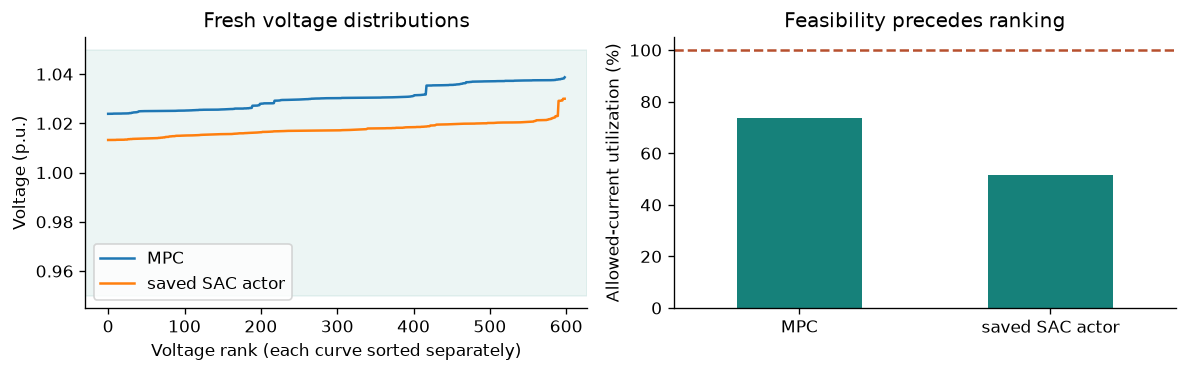
\includegraphics[width=.92\linewidth,height=3.25cm,keepaspectratio]{figures/classroom_voltage.png}
\end{center}
\begin{columns}[T]
\column{.48\textwidth}
\begin{tabular}{lrr}
\hline
Fresh L2 default & $J$ & MV gate\\\hline
MPC & 0.031104 & PASS\\
Saved SAC actor & 0.436428 & PASS\\\hline
\end{tabular}
\column{.48\textwidth}
{\small $J$: current-step teaching cost. Both actions pass this reduced-model contract. The voltage curves are sorted separately: equal rank is not equal bus identity.}
\end{columns}
\uncover<2->{\VoltageIdea{Attribute the result correctly}{The cost gap is a controller result. It does not, by itself, measure the benefit of agent orchestration.}}

\Source{Executed \texttt{Classroom\_Labs.ipynb}; \texttt{src/classroom\_labs.py}}
\Bridge{What can a language model add after numerical evidence already exists?}
\note{Use the actual executed L2 figure. The displayed default costs are rounded for teaching: MPC is approximately 0.031104 and SAC 0.436428, with both feasible under the reduced-model contract. The voltage curves are sorted separately, so matching positions are ranks rather than the same physical bus. The current-utilization plot reports the most heavily used allowed current bound. Ask participants to identify the evidence for feasibility before comparing objective values. A cost gap here is a controller result, not automatically an advantage of the multi-agent architecture. Students with changed load settings should report their own values and avoid mixing them with this original reference output.}
\end{frame}

\begin{frame}[t]{L3 opens a different, explicitly archived context}
\label{f:V17}
\small

\Checkpoint{L3}{Inspect original \texttt{test\_01}; these are actual recorded model responses.}
\begin{columns}[T]
\column{.53\textwidth}
\lstinputlisting[style=python,firstline=1,lastline=8]{snippets/L3.py}
\column{.44\textwidth}
\par\begin{tikzpicture}[node distance=7mm]
\node[box,text width=4.5cm] (live) {L2: fresh classroom scenario\\possibly edited by you};
\node[box,fill=amber!15,text width=4.5cm,below=of live] (arc) {L3: original archived test 01\\saved model replies + context};
\draw[red,thick,dashed] (live.south)--node[right,font=\scriptsize,text=red]{not automatically refreshed}(arc.north);
\end{tikzpicture}\par
\medskip
\uncover<2->{\VoltageIdea{Read the provenance}{
\texttt{reason}: exact public response.\\
\texttt{seconds}: recorded call time.\\
Printing the table makes no new LLM call.}}
\end{columns}

\Source{Executed \texttt{Classroom\_Labs.ipynb}; \texttt{src/classroom\_labs.py}; Recorded \texttt{LLM\_Response\_Selection.ipynb}; raw calls in \texttt{results/ensemble\_voltage\_pilot/}}
\Bridge{Do the actual explanations support the physical claims they make?}
\note{Explain why this cell is reproducible without contacting a local model. It loads an archived response pool from original test\_01, displays each exact public response and reports how the structured proposals were canonicalized. The seconds column contains recorded call durations, not the time required to print the table. The original test context is not identical to L2's default rating fraction, and certainly not to a student-modified L2 scenario. This cell therefore teaches inspection and evidence attribution. It does not supply new context-matched recommendations for the latest classroom perturbation. Ask learners to find a claim in a reason that is supported by the numeric evidence and one that still requires testing.}
\end{frame}

\begin{frame}[t]{Read the actual replies, then challenge their claims}
\label{f:V18}
\small

{\small Exact public excerpts, archived original test 01. Llama is the model family; Ollama is the local runtime.}
\medskip
\begin{columns}[T]
\column{.32\textwidth}
\VoltageIdea{Llama 3.1 8B \quad 1.867 s}{Trial: increase $a$ by 0.0025.}
{\small\itshape Increasing active participation by 0.0025 may help reduce curtailment and improve the overall performance.}
\column{.32\textwidth}
\VoltageIdea{Llama 3.2 3B \quad 0.905 s}{Trial: reduce $|b|$ by 10\%.}
{\small\itshape Reducing reactive effort magnitude by ten percent may help improve the overall system performance and reduce curtailment}
\column{.32\textwidth}
\VoltageIdea{Qwen 2.5 7B \quad 1.844 s}{Trial: reduce $|b|$ by 10\%.}
{\small\itshape may help improve voltage stability without significantly degrading active power performance}
\end{columns}
\medskip
\uncover<2->{\Question{Which phrases need evidence beyond a plausible explanation?}}
\uncover<3->{\begin{columns}[T]
\column{.48\textwidth}\VoltageIdea{Reactive effort $\ne$ curtailment}{Reducing $|b|$ does not itself prove higher active generation.}
\column{.48\textwidth}\VoltageIdea{Snapshot $\ne$ stability proof}{Steady-state power flow does not establish voltage stability.}
\end{columns}}

\Source{Recorded \texttt{LLM\_Response\_Selection.ipynb}; raw calls in \texttt{results/ensemble\_voltage\_pilot/}}
\Bridge{How do we compare three replies as physical actions?}
\note{These times and choices come from the recorded response-selection pilot. Llama 3.1 suggested increasing active participation to reduce curtailment. Llama 3.2 described reducing reactive effort and also mentioned reducing curtailment, a causal connection that its text alone does not establish. Qwen used the phrase voltage stability, which is unsupported by these steady-state tests. Present the excerpts as public rationales, not access to private model reasoning. Llama names the model family; Ollama is the local runtime that served it. Have the audience annotate the difference between a permitted operation and a justified physical claim. The next step converts prose-backed choices into reproducible physical candidates.}
\end{frame}

\begin{frame}[t]{Canonicalize actions before counting votes}
\label{f:V19}
\small

\begin{center}
\par\begin{tikzpicture}[x=1cm,y=1cm]
\node[box,text width=2.1cm] (l1) at (0,1.25) {Llama 3.1\\PV increase};
\node[box,text width=2.1cm] (l2) at (0,0) {Llama 3.2\\Q reduction};
\node[box,text width=2.1cm] (qw) at (0,-1.25) {Qwen 2.5\\Q reduction};
\node[box,text width=2.7cm] (pv) at (4,1) {Candidate A\\$(a+0.0025,b)$\\one vote};
\node[box,fill=teal!15,text width=2.7cm] (qr) at (4,-1) {Candidate B\\$(a,0.9b)$\\two votes};
\draw[arrow] (l1)--(pv);\draw[arrow] (l2)--(qr);\draw[arrow] (qw)--(qr);
\uncover<2->{\node[box,text width=2.6cm] (sel) at (8,0) {Select B\\for one numerical trial};
\draw[arrow,draw=amber] (qr)--(sel);}
\uncover<3->{\node[box,fill=amber!15,text width=2.6cm] (check) at (8,-1.8) {Simulate and verify};
\draw[arrow,draw=amber] (sel)--(check);}
\end{tikzpicture}\par
\end{center}
{\small $a,b$: incumbent fleet command. Tool name and parameters identify the same physical operation; prose style does not create a new action.}
\VoltageIdea{A majority is a selection rule}{Correlated language models can share an error. Agreement is not a calibrated probability of safety.}

\Source{Recorded \texttt{LLM\_Response\_Selection.ipynb}; raw calls in \texttt{results/ensemble\_voltage\_pilot/}}
\Bridge{Can experience improve the choice of which candidate to test?}
\note{Animate three response cards merging into two physical-candidate cards. Two different descriptions of the same command must not count as two distinct control actions. Canonical identifiers depend on the tool and parameters rather than rhetorical style. In original test\_01, two models propose the same reactive reduction and one proposes a PV increase, so the majority chooses the reactive trial. A predetermined hash tie-break makes ties reproducible; it is not an engineering preference. Agreement is also not a calibrated safety probability because models can share mistaken assumptions. A changed command returns to the numerical stages. Ask what should happen if the majority-selected trial fails a current constraint.}
\end{frame}

\begin{frame}[t]{LinUCB learns which proposed operation is worth testing}
\label{f:V20}
\small

\begin{columns}[T]
\column{.40\textwidth}
\par\begin{tikzpicture}[node distance=5mm]
\node[box,text width=4.6cm] (x) {Context + canonical operation\\features $\phi(s,o)$};
\node[box,text width=4.6cm,below=of x] (q) {Predict reward\\and explore during training};
\node[box,text width=4.6cm,below=of q] (r) {Test selected operation\\observe numerical reward};
\draw[arrow] (x)--(q);\draw[arrow] (q)--(r);
\uncover<2->{\draw[arrow,draw=amber] (r.west)--++(-.5,0)|- (q.west);}
\end{tikzpicture}\par
\column{.57\textwidth}
\begin{align*}
q(o\mid s)={}&
\underbrace{\theta^\top\phi(s,o)}_{\text{predicted reward}}\\
&+\underbrace{\beta\sqrt{\phi(s,o)^\top A^{-1}\phi(s,o)}}_{\text{training exploration bonus}},\\
o^*={}&\arg\max_o q(o\mid s).
\end{align*}
{\small $s$: evidence context; $o$: canonical operation; $\phi$: features; $\theta$: learned coefficients; $A$: regularized feature information; $\beta$: exploration weight; $q$: score; $o^*$: selected operation.}
\end{columns}
\uncover<3->{\VoltageIdea{Frozen classroom evaluation}{Use predicted reward only, with no updates. All LLM replies already exist: this learner does not choose which model to call or train LLM weights.}}

\Source{\href{https://arxiv.org/abs/1003.0146}{Li et al.: LinUCB, WWW 2010}; Recorded \texttt{LLM\_Response\_Selection.ipynb}; raw calls in \texttt{results/ensemble\_voltage\_pilot/}}
\Bridge{What should happen when a high predicted reward fails the physical gate?}
\note{Explain select, observe and update before revealing the formula. The feature vector represents the known context and a canonical operation, including vote-related information. Theta stores learned reward coefficients; A stores regularized feature information. During training, beta controls an uncertainty bonus. After a trial, selected feedback updates the reward model. The classroom evaluation freezes these parameters and uses predicted reward only, with no test updates. All candidate LLM responses have already been generated, so their call costs are paid by every pool selector. This is a contextual bandit, a simple reinforcement-learning setting, rather than training the language models or adapting a full sequential control policy online.}
\end{frame}

\begin{frame}[t]{Reward learning and physical acceptance have different jobs}
\label{f:V21}
\small

\[
r=\begin{cases}
\displaystyle
\min\!\left(1,\frac{\max(0,J_{\rm inc}-J_{\rm trial})}{0.01}\right)-0.01,
&\text{trial passes},\\[2mm]
-1.01,&\text{trial rejected}.
\end{cases}
\]
{\small $r$: post-trial reward; $J_{\rm inc},J_{\rm trial}$: incumbent and trial current-step costs. The 0.01 charge is a fixed trial penalty, \emph{not seconds}.}
\medskip
\begin{center}
\par\begin{tikzpicture}[x=1cm,y=1cm]
\node[box,text width=2.9cm] (tr) at (0,0) {24 training contexts\\selected feedback updates};
\node[box,text width=2.9cm] (va) at (4.1,0) {8 validation contexts\\frozen};
\node[box,text width=2.9cm] (te) at (8.2,0) {12 held-out test contexts\\frozen};
\draw[arrow] (tr)--(va);\draw[arrow] (va)--(te);
\end{tikzpicture}\par
\end{center}
\uncover<2->{\Question{The learner predicts improvement, but the trial violates current. Accept?}
\Answer{Reject the trial. Keep a valid incumbent or escalate; reward does not grant permission.}}

\Source{\href{https://arxiv.org/abs/1003.0146}{Li et al.: LinUCB}; Recorded \texttt{LLM\_Response\_Selection.ipynb}; raw calls in \texttt{results/ensemble\_voltage\_pilot/}}
\Bridge{Does the frozen choice agree with the majority and pass a new check?}
\note{Read the reward in two branches. A passing trial can earn a bounded improvement reward relative to the incumbent cost, with a fixed trial charge. A rejected trial receives a negative reward. The 0.01 scaling and charge are design choices; the charge does not measure latency. Training consumes selected outcomes, although the audit records contain other outcomes for comparisons. Validation and test are frozen, avoiding feedback leakage. Five training orders reuse the same training contexts and are not five independent datasets. Ask learners how changing reward scaling might change selection without changing any electrical operating limit. This separates learning preferences from the hard verification contract.}
\end{frame}

\begin{frame}[t]{L4: verify the frozen choice with a new numerical trial}
\label{f:V22}
\small

\Checkpoint{L4}{Three minutes: run the full cell and explain the output.}
\begin{columns}[T]
\column{.59\textwidth}
\lstinputlisting[style=python,firstline=1,lastline=8]{snippets/L4.py}
\column{.38\textwidth}
\VoltageIdea{Before the trial}{Which canonical operation did the learner choose? Does it match the majority?}
\medskip
\uncover<2->{\VoltageIdea{After the trial}{Did the fresh gate pass? What current-step cost was obtained?}}
\medskip
\uncover<3->{\textbf{Default:} learner and vote select Q reduction; original-context $J\approx0.031082$.}
\end{columns}
\medskip
{\small This evaluates archived original choices in their original context. Do not subtract this cost from a changed L2 scenario's cost.}

\Source{Executed \texttt{Classroom\_Labs.ipynb}; \texttt{src/classroom\_labs.py}; Recorded \texttt{LLM\_Response\_Selection.ipynb}; raw calls in \texttt{results/ensemble\_voltage\_pilot/}}
\Bridge{Does learned selection beat a simpler supervisor across held-out cases?}
\note{Read the exact L4 code, then give participants three minutes. The stored selector chooses an operation using its frozen parameters. The numerical helper evaluates the selected trial again under the archived original context. The displayed predicted reward is a learned estimate, while the returned trial table contains newly calculated outcomes. Participants should check whether the canonical candidate matches the majority choice and whether it passes the engineering gate. In this recorded test, the learner and majority agree on reactive reduction. Do not subtract this cost from a modified L2 cost, because those are different contexts. Ask which outcome controls the recommendation if a predicted improvement conflicts with failed verification.}
\end{frame}

\begin{frame}[t]{A fair experiment can find no learned advantage}
\label{f:V23}
\small

{\small Recorded held-out MV pilot: 12 scenarios; lower $J$ is better under the same reduced-model contract.}
\medskip
\begin{center}
\begin{tabular}{lrr}
\hline
Selection method & Mean $J$ & Same-action full AC PASS\\\hline
Fixed numerical refinement & 0.03400656 & 0/12\\
Majority vote & 0.03398479 & 0/12\\
Frozen learned selector & 0.03398479 & 0/12\\\hline
\end{tabular}
\end{center}
\uncover<2->{\begin{columns}[T]
\column{.48\textwidth}\VoltageIdea{Observed}{Vote and learner tie on every held-out case.}
\column{.48\textwidth}\VoltageIdea{Diagnostic}{A posthoc fixed Q-reduction rule reproduces their choices without LLM calls.}
\end{columns}}
\uncover<3->{\VoltageIdea{What this supports}{Reproducible trials and explicit checking are demonstrated. Superior control from extra LLMs or a learned selector is not established.}}

\Source{Recorded \texttt{LLM\_Response\_Selection.ipynb}; raw calls in \texttt{results/ensemble\_voltage\_pilot/}}
\Bridge{How much additional decision time did the response pool require?}
\note{Present this result without framing a tiny cost change as general superiority. The majority vote and frozen learner tie on all twelve held-out MV cases. A simple posthoc rule that always selects the reactive reduction reproduces those choices without language-model calls. Because that rule was identified after inspecting results, label it a diagnostic rather than a predeclared baseline. The experiment demonstrates that bounded proposals, fresh verification and reproducible traces can be implemented. It does not demonstrate that additional LLMs or a learned selector are necessary for better control. Ask what new test set or task distribution would make the learner's contribution more convincing than the simpler supervisor.}
\end{frame}

\begin{frame}[t]{Report the latency of the entire decision path}
\label{f:V24}
\small

\begin{center}
\par\begin{tikzpicture}[x=.85cm,y=1cm]
\draw[arrow] (0,0)--(9.7,0) node[right,font=\small]{seconds};
\foreach \x in {0,2,4,6,8}{\draw[slate] (\x,0)--(\x,-.1);\node[below,font=\small] at (\x,-.1){\x};}
\node[left,font=\small,align=right] at (0,1) {Fixed numerical\\refinement};
\fill[teal!75] (0,.7) rectangle (3.327,1.3);
\node[right,font=\small] at (3.327,1){3.327 s};
\uncover<2->{\node[left,font=\small,align=right] at (0,2.1) {Learned selector\\with response pool};
\fill[amber!85] (0,1.8) rectangle (8.119,2.4);
\node[right,font=\small] at (8.119,2.1){8.119 s};}
\end{tikzpicture}\par
\end{center}
{\small Recorded component times, reconstructed serial accounting for the held-out MV pilot. These are not guarantees for a deployed control room.}
\medskip
\begin{columns}[T]
\column{.48\textwidth}\VoltageIdea{Count all work}{Every pool selector pays for all three LLM responses, plus numerical trials and checks.}
\column{.48\textwidth}\VoltageIdea{Separate timing boundaries}{Training, model loading, token generation, actor inference and end-to-end execution are different quantities.}
\end{columns}

\Source{Recorded \texttt{LLM\_Response\_Selection.ipynb}; raw calls in \texttt{results/ensemble\_voltage\_pilot/}; \href{https://docs.ollama.com/api/chat}{Ollama chat API timing fields}}
\Bridge{What happens when the same chosen action is tested by a broader model?}
\note{The two reported times are reconstructed serial accounting from actual recorded components in the held-out pilot. They are not a guaranteed deployment response time and should not be confused with a new classroom timing measurement. Pool-based selectors share the cost of generating the three responses. The learned selector's small scoring operation is only one component of that total. Cold model loading, prompt processing, token generation and numerical checking can have very different scaling. Ask learners to draw the boundary around the quantity they want to compare. The engineering question is whether any incremental benefit justifies the additional decision latency under the intended operator workflow.}
\end{frame}

\begin{frame}[t]{L5 separates same-action auditing from AC replanning}
\label{f:V25}
\small

\Checkpoint{L5}{Default: fresh MV audit. Optional: full AC audit and a separate AC MPC solve.}
\begin{columns}[T]
\column{.54\textwidth}
\lstinputlisting[style=python,firstline=1,lastline=6]{snippets/L5.py}
{\small Enable \texttt{RUN\_OPENDSS} in L0 for the optional path. Run OpenDSS evaluations sequentially.}
\column{.43\textwidth}
\par\begin{tikzpicture}[node distance=7mm]
\node[box,text width=4.4cm] (u) {Existing MV-planned command};
\node[box,fill=amber!15,text width=4.4cm,below=of u] (a) {OpenDSS audit\\same action, broader coverage};
\draw[arrow] (u)--(a);
\uncover<2->{\node[box,text width=4.4cm,below=of a] (m) {Separate AC MPC solve\\new action using broader model};
\draw[arrow,draw=amber] (a)--(m);}
\end{tikzpicture}\par
\end{columns}
\uncover<3->{\VoltageIdea{Two questions}{Does the old recommendation survive the audit? What would a planner using the broader model recommend instead?}}

\Source{Executed \texttt{Classroom\_Labs.ipynb}; \texttt{src/classroom\_labs.py}; \href{https://opendss.epri.com/}{EPRI OpenDSS documentation}}
\Bridge{Which model actually checks the requested operating scope?}
\note{Read the helper call before enabling its optional path. The same-action audit asks whether an existing recommendation survives a broader physical model. The separate AC MPC solve asks what command a planner using that broader model would propose. Mixing those questions can make model coverage look like an LLM improvement. The default classroom execution performs the MV check; enabling RUN\_OPENDSS in L0 requests the fresh AC audit and separate AC replanning in L5. The saved learner remains frozen. OpenDSS computations should be performed sequentially because the local engine has shared mutable state. Compare the status, limiting quantities and model scope rather than treating cross-model costs as an exact solver ranking.}
\end{frame}

\begin{frame}[t]{A reduced-model PASS can fail the full-feeder audit}
\label{f:V26}
\small

\begin{center}
\par\begin{tikzpicture}[x=1cm,y=1cm]
\node[box,text width=2.8cm] (u) at (0,0) {MV-planned actions\\12 paired scenarios};
\node[box,fill=teal!15,text width=3.3cm] (mv) at (5,1) {MV gate\\12/12 PASS};
\node[box,fill=red!8,text width=3.3cm] (ac) at (5,-1) {Same-action AC audit\\0/12 PASS};
\draw[arrow] (u)--(mv);
\draw[arrow,draw=red] (u)--(ac);
\uncover<2->{\node[box,fill=teal!15,text width=3.2cm] (new) at (10,-1) {AC-planned final actions\\12/12 AC PASS};
\draw[arrow,draw=amber] (ac)--node[above,font=\scriptsize]{replan}(new);}
\end{tikzpicture}\par
\end{center}
\begin{columns}[T]
\column{.48\textwidth}\VoltageIdea{What changed}{Numerical equations and network/constraint coverage. The selector remained frozen.}
\column{.48\textwidth}\VoltageIdea{What did not follow}{This does not prove an LLM caused the better physical result, nor does PASS constitute human approval.}
\end{columns}
{\small Separately recorded 12-case pilot; not the output of one classroom L5 execution.}

\Source{Recorded \texttt{LLM\_Response\_Selection.ipynb}; raw calls in \texttt{results/ensemble\_voltage\_pilot/}}
\Bridge{With the broader model held fixed, does learned selection improve cost?}
\note{The table summarizes the separately recorded twelve paired scenarios, not the output of one L5 cell. The reduced model accepts all twelve final actions under its own scope, yet their same-action full-feeder audits fail. Planning with the AC backend returns actions that pass the full-feeder snapshot contract in these scenarios. The result is caused by the broader model and constraint coverage, with the selector still frozen. It cannot be attributed to more convincing Llama explanations. Within the AC pilot, the learned selector also does not establish superiority over fixed or uniform selection. Ask learners how a responsible operator packet should describe an MV-only recommendation when full MV/LV coverage was requested.}
\end{frame}

\begin{frame}[t]{The AC comparison still needs a strong numerical baseline}
\label{f:V27}
\small

\begin{columns}[T]
\column{.52\textwidth}
{\small Recorded paired AC pilot, 12 scenarios.}
\medskip
\begin{tabular}{lr}
\hline
Method & Mean current-step $J$\\\hline
MPC first action & 0.47172417\\
Fixed refinement & 0.47112138\\
Uniform pool selection & 0.47110513\\
Majority vote & 0.47138488\\
Frozen learned selection & 0.47138488\\\hline
\end{tabular}
\column{.45\textwidth}
\VoltageIdea{Interpretation}{Vote and learner tie. The learned selector does not beat the fixed or uniform comparators here.}
\medskip
\uncover<2->{\VoltageIdea{Check the raw policy too}{Only 1/12 raw SAC actions passes the AC gate in this pilot. A fast proposal is not automatically usable.}}
\end{columns}
\uncover<3->{\VoltageIdea{Why this is a scientific result}{Hold scenario, feasible set, budget and evaluation boundary constant. Attribute changes to the controller, model, information or orchestration mechanism that actually changed.}}
{\small Do not compare AC and MV objective means as a pure solver ranking: the modeled voltage sets differ.}

\Source{Recorded \texttt{LLM\_Response\_Selection.ipynb}; raw calls in \texttt{results/ensemble\_voltage\_pilot/}}
\Bridge{What should the operator receive after this whole workflow?}
\note{The broader AC model improves the relevance of the checked constraint set, but that does not establish a benefit from the learned response selector. In the twelve paired AC scenarios, the frozen learner and majority vote tie, and their mean current-step cost is worse than the fixed-refinement and uniform-pool comparators. The raw SAC proposal passes only one of twelve AC checks in this pilot, illustrating transfer limitations. Explain that every listed final recommendation still needs its declared physical gate. Do not compare the AC mean directly with the MV mean as if they measured an identical voltage set. A rigorous architecture study isolates the contribution of each changed component and reports negative results alongside successes.}
\end{frame}

\begin{frame}[t]{The operator receives a scoped recommendation and its evidence}
\label{f:V28}
\small

\begin{columns}[T]
\column{.62\textwidth}
\begin{tabular}{p{2.0cm}p{6.0cm}}
\hline
Stage & Returned evidence in this lesson\\\hline
Awareness & Load, rating fraction, requested scope, revision\\[1mm]
Planning & MPC and SAC candidate commands\\[1mm]
Simulation & New voltages, currents and objective\\[1mm]
Verification & PASS / failures; candidate-bound model evidence\\[1mm]
LLM optimizer & Permitted trial and recorded public rationale\\\hline
\end{tabular}
\column{.35\textwidth}
\par\begin{tikzpicture}[node distance=7mm]
\node[box,text width=4cm] (pk) {Command + model scope\\checks + limitations};
\node[box,fill=amber!15,text width=4cm,below=of pk] (h) {Human reviews\\and reads back the ID};
\draw[arrow] (pk)--(h);
\end{tikzpicture}\par
\uncover<2->{\medskip\VoltageIdea{Full scope requested?}{An MV-only PASS remains HOLD for a request requiring full MV/LV coverage.}}
\end{columns}
\uncover<3->{\VoltageIdea{Demonstrated benefit and boundary}{The workflow makes assumptions, trials and failures inspectable. Extra LLMs did not demonstrate better control here. Readback is advisory, not equipment dispatch.}}

\Source{Executed \texttt{Classroom\_Labs.ipynb}; \texttt{src/classroom\_labs.py}, L1--L5 and L12; Recorded \texttt{LLM\_Response\_Selection.ipynb}; raw calls in \texttt{results/ensemble\_voltage\_pilot/}}
\Bridge{After the break: what changes when the action is a topology rather than a setpoint?}
\note{Close the voltage chapter with the complete path and the actual findings. The numerical controllers supplied proposed settings. The language models supplied bounded refinement choices and public explanations. Voting and frozen learned selection tied in the held-out MV pilot. Broader-model checking revealed that the reduced-model recommendations did not meet the requested full-feeder scope. These are valuable workflow lessons without a claim of universal agentic control superiority. The operator must see the command, scenario, evidence, failed checks, remaining assumptions and required scope. Readback remains advisory and does not dispatch equipment. Invite one participant to name a demonstrated benefit and another to name a limitation, then take the scheduled ten-minute break before restoration.}
\end{frame}



